%%%%%%%%%%%%%%%%%%%%%%%%%%%%%%%%%%%%%%%%%%%%%%%%%%%%%%%%%%%%%%%%%%%%%%
% Lớp 12 | Ứng dụng đạo hàm để khảo sát hàm số | Sự đồng biến và nghịch biến của hàm số
% Dạng 2D1?1-4: Ứng dụng tính đơn điệu để chứng minh bất đẳng thức, giải phương trình,
% Số câu: 2  (sinh tự động bởi tach_cau.py; từ nay thầy sửa trực tiếp file này)
%%%%%%%%%%%%%%%%%%%%%%%%%%%%%%%%%%%%%%%%%%%%%%%%%%%%%%%%%%%%%%%%%%%%%%

%%%%%%%%%%%%%%%% ĐÚNG/SAI %%%%%%%%%%%%%%%%

% nguồn: Phan1_Lop_12_Dai_so_Chuong_1
\begin{ex}%[2D1V1-4]%[ma:eedbd692]
	Cho hàm số  $f(x)=3x^3-7 x^2+5 x-6$.
	\choiceTF 
		{Hàm số đạt cực đại tại $x=1$ và  đạt cực tiểu tại $x=\dfrac{5}{9}$}
		{\True Hàm  số đồng biến trên khoảng $(-1;0)$}
		{Hai điểm cực trị của đồ thị hàm số nằm khác phía  so với trục $Ox$}
		{Tồn tại hai  số thực $a$, $b$ với $a<b$ sao cho $\log _{\tfrac{\pi}{4}}[f(a)]<\log _{\tfrac{\pi}{4}}[f(b)]$}
	 \loigiai{
		\begin{itemchoice}
			 \itemch
			Tập xác định $\mathscr{D} =\mathbb{R}$, ta  có $$f^{\prime}(x)=9 x^2-14 x+5
			 ,~f^{\prime}(x)=0 \Leftrightarrow\hoac{&
			x=1  \\&
			x=\dfrac{5}{9}.} 
			 $$
			 Bảng biến thiên
			\begin{center}
				\begin{tikzpicture}
					 \tkzTabInit[nocadre=false,lgt=1.2,
						espcl=4,deltacl=0.6] 
						{$x$/1.2,$y'$/0.6,$y$/3}{$-\infty$,$\dfrac{5}{9}$,$1$,$+\infty$} 
					 \tkzTabLine{,+,0,-,0,+,}
					\tkzTabVar{-/$-\infty$,+/$-\dfrac{1\,183}{243}$,-/$-5$,+/$+\infty$} 
				\end{tikzpicture}
			\end{center}
			Vậy hàm số đạt cực đại tại $x=\dfrac{5}{9}$, đạt  cực tiểu tại $x=1$.
			 \itemch
			Hàm số đồng biến trên $\left(-\infty;\dfrac{5}{9}\right)$ và $(1;+\infty)$ suy ra hàm  số đồng biến trên $(-1;0)$.\\
			\itemch Hàm số đạt cực đại tại $x=\dfrac{5}{9}$, giá trị cực đại $f\left(\dfrac{5}{9}\right)=-\dfrac{1\,183}{243}$. \\Hàm số đạt cực tiểu tại  $x=1$, giá trị cực tiểu $f(1)=-5$.\\
			Vì $f\left(\dfrac{5}{9}\right) \cdot f(1)>0$ nên hai điểm cực trị của đồ thị hàm số nằm cùng phía so  với trục $Ox$.
			\itemch Ta có $f(x)>0 \Leftrightarrow 3x^3-7 x^2+5  x-6>0 \Leftrightarrow x>2$ và trên $(2;+\infty)$ hàm số đồng biến.\\
			Suy ra $\heva{&f(a)>0 \\& f(b)>0}  \Leftrightarrow\heva{&a>2 \\& b>2.}$\\
			Ta có $$\log _{\tfrac{\pi}{4}}[f(a)]<\log _{\tfrac{\pi}{4}}[f(b)] \Leftrightarrow f(a)>f(b) \Leftrightarrow a>b$$ (trái với giả thiết), suy ra không tồn tại số thực $a, b$ thỏa  mãn đề bài.
		\end{itemchoice}
	} 
\end{ex}

% nguồn: Phan1_Lop_12_Dai_so_Chuong_1
\begin{ex}%[2D1V1-4]%[ma:fcdbe815]
	Tại thời điểm $t$  giờ kể từ khi tiêm một liều thuốc cho bệnh nhân, nồng độ thuốc trong máu được tính bởi công thức $C(t)=0{,}5 t e^{-0{,}5 t}$ $\mathrm{mg} / \mathrm{ml}$ (với $t \geq 0$).
	 \choiceTF
		{Ban đầu (tại thời điểm tiêm) nồng độ thuốc có trong máu bệnh  nhân là $0{,}5$ $\mathrm{mg/ml}$}
		{\True  Kể từ thời điểm $t=2$ (giờ), nồng độ thuốc trong máu bệnh nhân giảm dần}
		{Nồng độ thuốc trong máu có thể vượt quá $0{,}5$ $\mathrm{mg} / \mathrm{ml}$} 
		{\True Có thời  điểm nồng độ thuốc trong máu bằng $0{,}3$ $\mathrm{mg} / \mathrm{ml}$}
	\loigiai{ 
		\begin{itemchoice}
			 \itemch Sai. Do $C(0)=0$.
			\itemch  Đúng. Do
			 $C^{\prime}(t)=0{,}5 e^{-0{,}5 t}(1-0{,}5 t).\\
			C^{\prime}(t)=0 \Leftrightarrow t=2$. 
			\begin{center}
				\begin{tikzpicture}
					 \tkzTabInit[lgt=1.2,espcl=3]
						{$x$ /0.6,$f’(x)$ /0.6,$f (x)$  /2.0}
						 {$0$,$2$,$+\infty$}
					 \tkzTabLine{,+,0,-,}
					\tkzTabVar{-/$0$,+/$\dfrac{1}{\mathrm{e}}$,-/$0$} 
				\end{tikzpicture}
			\end{center}
			Vậy kể từ thời điểm $t=2$ (giờ), nồng độ thuốc trong máu bệnh  nhân giảm dần.
			\itemch Sai. Nồng độ thuốc trong máu không thể vượt  quá $0{,}5 \mathrm{mg} / \mathrm{ml}$\\
			(vì $\max  C(t)=C(2)=\dfrac{1}{e}<0{,}5$).
			\itemch Đúng. Có thời điểm nồng độ thuốc trong máu bằng $0{,}3 \mathrm{mg} / \mathrm{ml}$ (vì  $0<0{,}3<\dfrac{1}{e}$).
		\end{itemchoice}
	 }
\end{ex}
